% 1977 年陕西卷第十题图 2：圆与两边 AB、BC 相切于 E、F，且与内接正方形 A′B′C′D′ 的边 A′B′ 相切于 G
% （顶点标注按解答正文用 D′；源图该点印作 D，撇号系描图脱落）
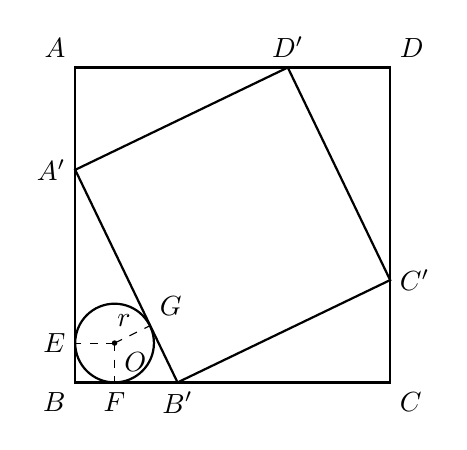
\begin{tikzpicture}[scale=1.0]
  \draw[thick] (0,0)--(4,0)--(4,4)--(0,4)--cycle;
  \draw[thick] (0,2.7)--(1.3,0)--(4,1.3)--(2.7,4)--cycle;
  \draw[thick] (0.5,0.5) circle (0.5);
  \draw[dashed] (0.5,0.5)--(0,0.5);
  \draw[dashed] (0.5,0.5)--(0.5,0);
  \draw[dashed] (0.5,0.5)--(0.95,0.72);
  \fill (0.5,0.5) circle (1pt) node[below right] {$O$};
  \node at (0.62,0.78) {$r$};
  \node[above right] at (0.95,0.72) {$G$};
  \node[left]  at (0,0.5) {$E$};
  \node[below] at (0.5,0) {$F$};
  \node[above left]  at (0,4)    {$A$};
  \node[left]        at (0,2.7)  {$A'$};
  \node[above]       at (2.7,4)  {$D'$};
  \node[above right] at (4,4)    {$D$};
  \node[right]       at (4,1.3)  {$C'$};
  \node[below left]  at (0,0)    {$B$};
  \node[below]       at (1.3,0)  {$B'$};
  \node[below right] at (4,0)    {$C$};
\end{tikzpicture}
